\chapter{Zestawienie zagadnień wykorzystanych w trakcie realizacj projektu}
\label{cha:Zestawienie zagadnień wykorzystanych w pracy}

\section{Mechaniczne układy napędowe}
%______________________________________________________________________________________________________________
\subsection{Przekładnie mechaniczne}
Układ napędowy to zestaw urządzeń wykorzystywany do napędzania, w skład którego wchodzi źrodło energii, układy pośredniczące w przekazywaniu energii oraz odbiornik energi. Mianem napędu zazwyczaj określa się urządzenia pośredniczące. Najczęściej wykorzystywanymi źródłami enrgii są silniki a odbirniki energii, których zadaniem jest realizowanie odpowiednich ruchów roboczych, przyjmują różne formy zależne od aplikacji.

Układ mechaniczny wykorzystany do przeniesienia ruchu obrotowego z elementu czynnego na element bierny nazywany jest przekładnią mechaniczną. Oprócz transmisji energii, przekładnie umożliwają również zmianę parametrów ruchu - momentu obrotowego oraz prędkości obrotowej. Przekładnie mechaniczne dzieli się na trzy grupy: cięgnowe, cierne i zębate. Przekładnie cięgnowe, które zostały opisane ze wzgędu na zastosowanie w rowerowych układach napędowych, składają się z conajmniej dwóch kół zębatych, rozsuniętych względem siebie, oraz cięgna opasającego. Ze względu na rodzaj zastosowanego cięgna, wyróżnia się przekładnie pasowe oraz łańcuchowe. Przenoszenie siły z cięgna na koło zębate jest możliwe dzięki zastosowaniu odpowiednich połączeń - połączenia cierne, kształtowe lub stałe przymocowanie cięgna do koła zębatego.

\textcolor{red}{@TODO wrzucić schemat przekładni, dodać jakiś przypis doprzełkadni}

Wielkością charakteryzującą przekładnie jest przełożenie. Wyróżnia się przełożenie geometryczne, kinematyczne oraz dynamiczne. Przełożenie kinematyczne to stosunek prędkości kątowej koła czynnego do prędkości kątowej koła biernego:
\textcolor{red}{@TODO wzorek i=w1/w2}

Przełożenie dynamiczne określa stosunek momentu obrotowego na kole biernym do momentu obrotowego koła czynnego.  

\textcolor{red}{@TODO wzorek i=M2/M1}

Przełożenie przekładni jest parametrem bezwymiarwoym. Ze względu na wartość przełożenia przekładni wyróznia się:
\begin{itemize}
\item
Przekładnie przyspieszające lub tzw. multiplikatory. Przekładnie tego typu zwiększają prędkość kątową koła biernego względem prędkości kątowej koła czynnego przy jednoczesnym zmniejszeniu momentu obrotowego koła biernego względem momentu obrotowego koła czynnego. Przełożenie takiej przekładni jest liczbą z zakresu od 0 do 1.
\item
Przekładnie redukujące lub tzw. reduktory. Przekładnie tego typu działają w sposób odwrotny do przekładni przyspieszających - zmniejszają prędkość kątową koła biernego względem prędkości kątowej koła czynnego oraz zwiększają moment obrotowy koła biernego wzlgędem momentu obrotowego koła czynnego. Przełożenei przekładni redukującej jest zawsze większe od 1.
\end{itemize} 
%____________________________________________________________________________________________________________  
\subsection{Układ napędowy w rowerze}
W przypadku konwencjonalnego układu napędowego stosowanego w rowerach źródłem energii jest rowerzysta. Siła przyłożona do ramienia korby generuje moment obrotowy, który przenoszony jest, przy pomocy mechanizmu korbowego i łańcucha, na koło zębate na stałe przymocowoane do piasty tylnego koła. Moment obrotowy koła napędzającego powoduje powstanie sił obwodowych, składających się na siłę napędową, która wprawia rower w ruch postępowy.

Układ napędkowy roweru wykorzystanego w pracy składa się z mechanizmu korbowego z jednym kołem zębatym, łańcucha, kasety ośmiorzędowej oraz przerzutki tylnej. Koło zebate zamontowane w mechaniźmie korbowym ma 34 zęby. Kaseta składa się z ośmiu kół zębatych, których liczba zębów należy do zakresu od 11 do 32. Przekładnia zastosowana w rowerze, niezależnie od aktualnego biegu, ma zawsze charakter mulitiplikatora.

Tylna przerzutkau umożliwia zmianę przełożenia układu napędowego. Działa na zasadzie czworoboku przegubowego. Składa się z czterech członów połączonych przegubowo, tworzących zamknięty łańcuch kinamatyczny. Pozycja wózka przerzutki przymontowanego do jedenego z członów (Rys.\ref{fig:przerzutka}) utrzymywana jest dzięki zastosowaniu sprężyny napinającej oraz cięgna, połączonego z mechanizmem do zmiany przełożeń, zamontowanym w manetce. Dodatkowo przerzutka posiada mechanizm napinający łańcuch, tak aby zachować pełną funkcjonalność układu napędowego niezależnie od aktualnej pozycji wózka przerzutki. 
\begin{figure}[h]
    \centering
    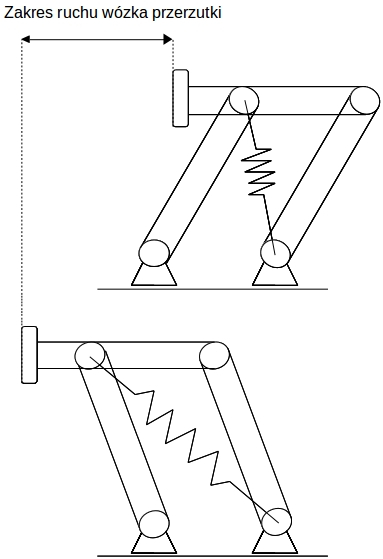
\includegraphics[scale=0.4]{przerzutka.jpg}
    \caption{Zasada działania konwencjonalnej przerzutki rowerowej}
    \label{fig:przerzutka}
\end{figure}
%____________________________________________________________________________________________________________ 

\section{Zagadnienia z Automatyki}
%____________________________________________________________________________________________________________  
\subsection{Zamknięty układ regulacji}
%____________________________________________________________________________________________________________
\subsection{Transmitancja operatorowa}

%____________________________________________________________________________________________________________  
\subsection{Serwomechanizm}
%____________________________________________________________________________________________________________  
\subsection{Filtr donlnoprzepustowy RC}
\label{filtrRc}
%____________________________________________________________________________________________________________  
\section{Metody pomiarowe wielkości fizycznych}
\subsection{Pomiar prędkości kątowej koła napędowego oraz prędkości liniowej roweru}

Możliwość pomiaru prędkości kątowej jest kluczowa ze względu na wykonanie trybu automatycznej zmiany przełożeń. Na podstawie aktualnej prędkości kątowej tylnego koła wyznaczona zostanie chwilowa prędkość liniowa. Pomiar prędkości kątowej mechanizmu korbowego umożliwi wyznaczenie aktulane wartości kadencji.

Prędkość kątowa jest wielkością wektorową, jednak w rozważaniach dotyczących pracy brana pod uwagę jest jedynie chwilowa wartość prędkości kątowej. Ta zdefiniowana jest jako zmiana drogi kątowej w czasie:
\begin{equation}
    \omega = \frac{d\varphi}{dt}
    \label{eq:predkoscKatowa}
\end{equation}
\begin{eqwhere}[2cm]
	\item[$\varphi$] droga kątowa
	\item[$t$] czas
\end{eqwhere}
Wyznaczenie chwilowej wartości prędkości kątowej wykonane zostało w oparciu o czujniki zbliżeniowy załączany magnetycznie, który został na stałe przymocowany do ramy roweru, w niewielkiej odległości do tylnego koła. Zasada działania takiego czujnika jest analogiczna do działania zwykłego przycisku monostabilnego. Obwód w czujniku jest domyślnie rozwarty. Zwarcie następuje w momencie zbliżenia magnesu do czujnika. Magnes przyczepiony został do szprychy roweru. Taki sam sposób pomiaru prędkości można znaleźć w komercyjnych licznikach rowerowych oferowanych na rynku. Autor zdecydował się na zastosowanie dwóch magnesów w celu zwiększenia dokładności pomiaru. Dysponując pomiarem czasu pomiędzy kolejnymi zwarciami czujnika magnetycznego, które, ze względu na zastosowanie dwóch magnesów, następują w wyniku obrotu koła o kąt $\pi$ , można wyznaczyć chwilową wartość prędkości kątowej: 
\begin{equation}
    \omega = \frac{\pi}{T}
\end{equation}
\begin{eqwhere}[2cm]
	\item[$T$] czas od ostatniego zwarcia czujnika magnetycznego
\end{eqwhere}
Prędkość kątowa mechanizmu korbowego została wyznaczona w sposób analogiczny. Zbliżeniowy czujnik magnetyczny, który został na stałe przymocowany do ramy roweru, w bliskiej odległości mechanizmu korbowego, jest zwierany w każdym cyklu dzięki zastosowaniu magnesu, który został przyklejony do ramienia mechanizmu korbowego. Ze względu na zastosowanie jednego magnesu, przyrost drogi kątowej jest dwa razy większy, niż w przypadku pomiaru prędkości kątowej koła roweru i jego wartość wynosi 2$\pi$.

Wartość prędkości liniowej to stosunek przebytej drogi do czasu:
\begin{equation}
    v = \frac{s}{t}
\end{equation}
\begin{eqwhere}[2cm]
	\item[$s$] droga liniowa
	\item[$v$] prędkość liniowa
\end{eqwhere}
 Związek pomiędzy drogą liniową a drogą kątową wyraża się wzorem:

\begin{equation}
    \varphi = \frac{s}{r}
\end{equation}

\begin{eqwhere}[2cm]
	\item[$r$] promień okręgu
\end{eqwhere}
W układzie pomiarowym z dwoma magnesami, wartość drogi kątowej w momencie zwarcia czujnika magnetycznego wynosi $\pi$. Biorąc pod uwagę powyższe zależnosci, chwilowa wartość prędkości liniowej poruszającego się roweru może zostać wyznaczona z zależności:
 \begin{equation}
    \label{eq:zaleznoscNaPredkosc}
    v = \frac{\pi R}{T}
\end{equation}
\begin{eqwhere}[2cm]
	\item[$R$] promień koła rowerowego
\end{eqwhere}
%____________________________________________________________________________________________________________  
\subsection{Inercyjna jednostka pomiarowa IMU}
Inercyjna jednostka pomiarowa ( z ang. {\em Inertial Measurement Unit}) to układ składający się z kilku czujników pomiarowych, pozwalających wyznaczyć orientację obiektu w przestrzeni trójwymiarowej. Stosowane m.in. w systemach stabilizacji bezzałogowych statków powietrznych. W realizowanym projekcie wykorzystana zostanie możliwość wyznaczenia kąta nachylenia podłoża, po którym porusza się rower z zamontowaną jednostką pomiarową IMU.

Jednostki IMU zazwyczaj wyposażone są w trzyosiowy akcelerometr, trzyosiowy żyroskop oraz magnetometr. Wszystkie czujniki to urządzenia wykonane w miniaturowej skali oraz technologii MEMS ( z ang. {\em Micro Electro-Mechanical Systems}), które integrują ze soba elementy mechaniczne oraz elektroniczne. Wykorzystywane głównie jako czujniki przetwarzające wielkości mechaniczne na wielkości elektryczne. Czujniki wykonane w technologii MEMS posiadają kilka znaczących zalet, które sprawiają, że spektrum zastosowań staje się coraz szersze. Są to m.in. niska cena, niewielkie rozmiary, niskie zużycie energii oraz prosta integracja z układami mikroprocesorowymi. 

%____________________________________________________________________________________________________________  
\subsubsection{Pomiar przyspieszeń - akcelerometr}
Akcelereometr to urządzenie pomiarowe, które umożliwia pomiar przyspieszenia dynamicznego ciała, na które działa niezerowa siła wypadkowa, oraz przyspieszenia statycznego ciała znajdującego się w ziemskim polu grawitacyjnym. Akcelerometry zazwyczaj działają na zasadzie przetworników pojemnościowych. Pomiar dokonywany jest dzięku zastosowaniu kondensatorów różnicowych, których ruchome okładki wychylane są z położenia równowagi pod wpływem działających sił bezwładności.

Akcelerometry są powszechnie wykorzystywane w różnego rodzaju aplikacjach. Układy sterujące poduszkami powietrznymi, systemy alarmowe w samochodach czy tzw. asysten ruszania na wzniesieniu to tylko niektóre przykłady z branży motoryzacyjnej.

Akcelerometr wykonany w technologii MEMS zazwyczaj umożliwia pomiar przyspieszenia w trzech różnych kierunkach(\textcolor{red}{@TODO rysunek}). Akcelerometr został zamontowany w rowerze w taki sposób, aby kierunek osi \textit{X} był równoległy do podłoża. Dzięki temu wskazania akcelerometru wzdłuż osi \textit{X} są proporcjonalne do siły wypadkowej działającej na rower.
%____________________________________________________________________________________________________________  
\subsubsection{Pomiar prędkości kątowych - żyroskop}
Żyrosko to urządzenie pomiarowe dostarczające informacji na temat chwilowej prędkości obrotowej układu pomiarowego. Żyroskopy wykonane w technologii MEMS to czujniki pojemnościowe wykorzystujące efekt Coriolisa. Układ dwóch wybrujących mas, umieszczony na obrotowej tarczy, zmienia swoje położenie względem osi obrotu w zależności od chwilowej prędkości obrotowej. W wyniku zmiany położenia układu mas odkształceniu ulega tarcza, która stanowi okładkę kondensatora. W efekcie następuje różnicowa zmiana pojemności kondensatora, która przetwarzana jest na chwilową prędkość obrotową.

Żyroskop, podobnie jak akceleorometr, to układ trzech czujników pozwajający na pomiar w trzech różnych kierunkach. Zamontowany został w taki sposób, aby kierunek osi żyroskopu \textit{X} oraz \textit{Z}  był równoległy do położa.

%____________________________________________________________________________________________________________  
\section{Estymata kąta nachylenia podłoża}
Kąt nachylenia podłoża, po którym porusza się rower, to ostatnia z wielkości  brana pod uwagę przez algorytm automatycznej zmiany przełożeń. Wielkość ta wyznaczona zostanie pośrednio, poprzez zastosowanie filtru komplementarnego wykorzystująecgo chwilowe wartości kąta nachylenia, wyznaczone na podstawie danych pochodzących z akcelerometru oraz żyroskpu.

%____________________________________________________________________________________________________________ 
\subsection{Analiza danych pomiarowych akcelerometru}
\label{pomiaryAkcel}
Przykład zamieszczony na rysunku \ref{fig:równia} przedstawia ciało znajdujące się na równi pochyłej. Przyspieszenie ziemskie \textit{$g$} zostało rozłożone na kierunki składowe wzdłuż osi pomiarowych akcelerometru - \textit{$a_x$} oraz \textit{$a_y$}. Wektory składowe wraz z przyspieszeniem ziemskim stanowią trójkąt podobny do trójkąta równi pochyłej, której kąt nachylenia został oznaczony jako $\alpha$. Stosunek długości przyprostokątnej leżącej naprzeciw kąta $\alpha$ do wartości drugiej przyprostokątnej, które odpowiadają wartością przyspieszeń mierzonym przez akcelerometr odpowiednio wzdłuz osi $x$ i $y$, wynosi $\tan{\alpha}$. Zastosowanie funkcji odwrotnej pozwala wyznaczyć kąt nachylenia równi:
\begin{equation}
    \alpha=\arctan{\frac{a_x}{a_y}}
    \label{eq:rowniaRadian}
\end{equation}
\begin{eqwhere}[2cm]
	\item[$\alpha$] kąt naychylenia podłoża
	\item[$a_x$] przyspieszenie akcelerometru mierzone wzłuż osi x
	\item[$a_y$] przyspieszenie akcelerometru mierzone wzłuż osi y
\end{eqwhere}
Zależność \ref{eq:rowniaRadian} pozwala wyznaczyć wartość miary łukowej kąta wyrażonej w radianach. W odniesieniu do kąta nachylenia podłoża po którym porusza się rower, zdecydowanie bardziej intuicyjną jednostką są stopnie. Przekształcenie miary kąta wyrażonej w radianach na miarę kąta wyrażoną w stopniach opisane jest poniższą zależnością:
\begin{equation}
    \alpha_{deg}=\frac{180\alpha}{\pi}
    \label{eq:rowniaStopnie}
\end{equation}
\begin{eqwhere}[2cm]
	\item[$\alpha_{deg}$] kąt naychylenia wyrażony w stopniach
\end{eqwhere}
\begin{figure}
    \centering
    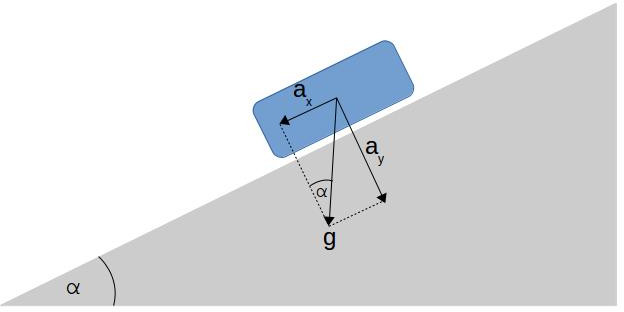
\includegraphics[scale=0.5]{katNachylenia.jpg}
    \caption{a nice plot}
    \label{fig:równia}
\end{figure}
%____________________________________________________________________________________________________________ 
\subsection{Analiza danych pomiarowych żyroskopu}
\label{gyro}
Zgodnie z zależnością \ref{eq:predkoscKatowa} prędkość kątowa określana jest jako zmiana drogi kątowej w czasie. Sytuacja odwrotna, czyli wyznaczenie drogi kątowej na podstawie pomiarów prędkości jest możliwe poprzez wyznaczenie funckji odwrotnej:
\begin{equation}  
    \varphi = \int\omega(t)dt
\end{equation}

Ta operacja została uwzględniona w projekcie filtru komplementarnego poprzez dodanie członu całkującego, którego transmitancja operatorowa wynosi $\frac{1}{s}$ - wzór \ref{eq:alpha} w pkt. \ref{kompZasadaDzialania}.

%____________________________________________________________________________________________________________ 
\subsection{Filtr komplementarny}
\label{kompZasadaDzialania}
Zasada działania filtru komplementarnego polega na odpowiedniej fuzji danych pochodzących z różnych czujników pomiarowych. Sygnał każdego z nich zawiera istotną informację o mierzonej wielkości jak również zakłócenia, które powinny zostać wyeliminowane. Fuzja danych polega na zastosowaniu odpowiednich filtrów, dolnoprzepustowych, środkowoprzepustowych i górnoprzepustowych, które eliminują zakłócenia charakterystyczne dla danego czujnika jednocześnie przuszczając informacje użyteczne. Warunkiem koniecznym uzyskania dokładniejszych wartości estymwoanych od wartości mierzonych jest zastosowanie czujników pomiarowych o różnej charakterystyce częśtotliwości błędów pomiarowych. Schemat przedstawiający ogólną idę filtru komplementarnego przedstawiony został na rys \ref{fig:kompGeneral}
\begin{figure}[h]
    \centering
    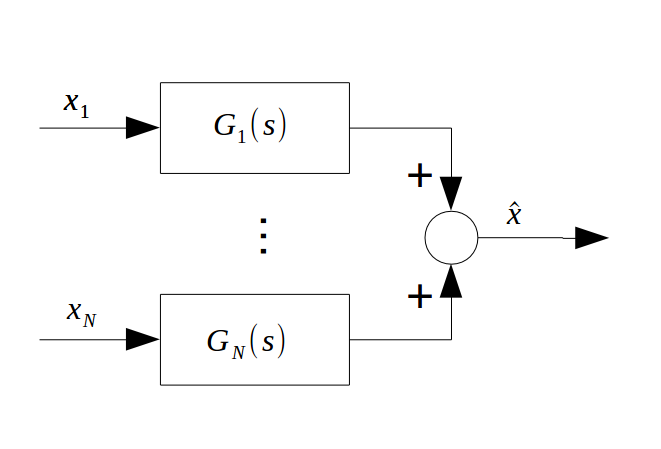
\includegraphics[scale=0.3]{filtrKomp.png}
    \caption{Zasada działania filtru komplementarnego. $x_1$ : $x_N$ - sygnały wejściowe, $G_1(s) : G_N(s)$ - transmitancje operatorowe poszególnych filtrów, $\hat{x}$ - estymowana wartość wyjściowa }
    \label{fig:kompGeneral}
\end{figure}

Zaprojektowany filtr nie powinien wprowadzać dodatkowej dynamiki - transmitancja operatorowa, określająca stosunek transformaty Laplace'a sygnału wyjściowego do transformaty Laplace'a sygnału wejściowego, powinna spełniać zależność:
\begin{equation}
    G(s)=\sum_{i=1}^{N}G_{i}(s)=1
    \label{eq:zasadaKomplementarnosci}
\end{equation}

W odniesieniu do estymacji wartości kąta nachylania podłoża, schmat filtru komplementarnego, wykorzystującego wartości kątów wyznaczonych na podstawie danych pomiarowych pochodzących z akcelerometru oraz żyroskopu, przedstawiony został na rys \ref{fig:kompKat}. 

Pomiar składowych przyspieszenia ziemskiego umożliwia wyznaczenie kąta nachylenia podłoża (pkt. \ref{pomiaryAkcel}). Ta metoda znajduje swoje zastosowanie wtedy, gdy układ pomiarowy nie porusza się lub porusza się ruchem jednostanym. W ruchu przyspieszonym dane pomiarowe akcelerometru uwzględniają siły powodujące ten ruch, a brak możliwości odseparowania składowych przyspieszenia ziemskiego sprawia, że kąt nachylenia obarczony jest błędem. Należy zastem zastosować filtr dolnoprzeustowy, eliminujący szybkozmienne wartości kąta nachylenia pochodzące z akcelerometru.

Żyroskop umożliwia pomiar prędkości obrotowej. Całkowanie prędkości obrotowej umożliwia wyznaczenie kąta nachylenia podłoża (pkt. \ref{gyro}). Jednak zakłócenia toru pomiarowego oraz wrażliwość na warunki pracy, a w szczególności temepraturę, powodują zjawisko tzw. dryfu żyroskopowego. Dryf spowodowany jest ciągłym narastaniem błędów w wyniku całkowania zakłóconych danych pomiarowyych. Błędy powstałe w wyniku dryfu żyroskopowego są sygnałami wolnozmiennymi. Zastosowanie filtru górnoprzepustowego pozwala je wyeliminować. 

Fliltr dolnoprzepustowy może zostać zrealizowany poprzez obiekt inercyjny I rzędu:
\begin{equation}
    G_{low}(s)=\frac{1}{Ts+1}
    \label{eq:lowPass}
\end{equation}
Zgodnie z równaniem \ref{eq:zasadaKomplementarnosci}, filtr górnoprzepustowy powinien spełniać zależność:
\begin{equation}
    G_{high}(s)=1-G_{1}(s)=\frac{Ts}{Ts+1}
    \label{eq:highPass}
\end{equation}
Transmitancja $G_{high}(s)$ odpowiada transmitancji filtru górnoprzepustowego RC.

\begin{figure}[h]
    \centering
    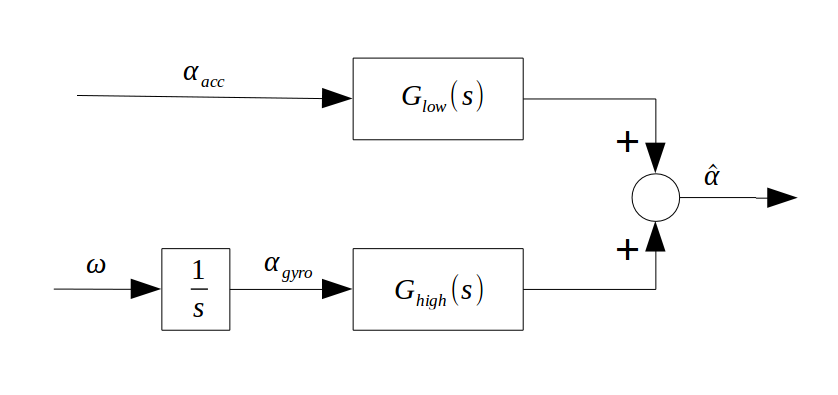
\includegraphics[scale=0.3]{filtrKompKat.png}
    \caption{Schemat filtru komplementarnego estymującego kąt nachylenia.}
    \label{fig:kompKat}
\end{figure}

Estymowana wartość kąta nachylenia $\hat{\alpha}$ spełnia zależność:
\begin{equation}
    \hat{\alpha} = \frac{1}{Ts+1}\alpha_{acc}+\frac{Ts}{Ts+1}\frac{1}{s}\omega = \frac{\alpha_{acc}+T\omega}{Ts + 1}
    \label{eq:alpha}
\end{equation}
\begin{eqwhere}[2cm]
	\item[$\hat{\alpha}$] estymata kąta nachylenia
	\item[$\alpha_{acc}$] kąt nachylania wyznaczony na podstawie danych z akcelerometru
	\item[$\omega$] prędkość obrotowa
\end{eqwhere}

Ze względu na potrzebę zaimplementowania filtru w układzie mikroprocesorowym, powyższe równanie należy zdyskretyzować w dziedzinie czasu. Można tego dokonać stosując metodę Eulera wstecz\textcolor{red}{GREGA przypis} jako przybliżenie operacji różniczkowania w czasie\textcolor{red}{sprawdz rownianei i dopisz oznaczenia, czy aby na pewno RÓŻNICZKOWANIA ?!}:
\begin{equation}
    s=\frac{t_0z}{z-1}
    \label{eq:eulerWstecz}
\end{equation}
\begin{eqwhere}[2cm]
	\item[$t_{0}$] długość kroku dyskretyzacji
\end{eqwhere}

Podstawiając zależność \ref{eq:eulerWstecz} do równania \ref{eq:alpha} równanie różnicowe estymujące wartość kąta nachylania podłoża przyjmuje postać:
\begin{equation}
    \hat{\alpha_{k}} = p(\hat{\alpha}_{k-1} + \omega_{k}t_0) + (1-p)\alpha_{acc}
\end{equation}
\begin{equation}
    p = \frac{T}{T + t_0}
\end{equation}
\begin{eqwhere}[2cm]
	\item[$t_{0}$] długość kroku dyskretyzacji
\end{eqwhere}
